% !TEX TS-program = xelatex
%
\documentclass{clseminar}

\usepackage[english]{babel}
\usepackage{parskip}

\usepackage{enumitem}

\usepackage{amsmath}
\usepackage{amssymb}
\usepackage{listings}

\usepackage{color}
\definecolor{red}{RGB}{200,50,0}
\definecolor{green}{RGB}{0,150,60}

\usepackage{tkz-graph}
\tikzset{vertex/.style = {shape=circle,draw,minimum size=1}}
\tikzset{edge/.style = {->,> = latex'}}

\title{Process Calculi for Concurrency}
\author{Markus Reiter, Michael Kaltschmid}
\supervisor{Vincent van Oostrom}

\begin{document}
  \abstract{Lorem ipsum dolor sit amet, consectetur adipiscing elit. Cras nisi purus, facilisis ut gravida ac, tempus iaculis risus. Vestibulum imperdiet condimentum risus non posuere. Praesent accumsan, metus nec dignissim porttitor, mi purus semper sem, id faucibus elit est vel felis. Orci varius natoque penatibus et magnis dis parturient montes, nascetur ridiculus mus. Cras at gravida ante. Nullam eu ex augue. Fusce ut enim vel tortor gravida egestas sit amet non risus. Sed semper iaculis eros, in feugiat arcu. Ut sit amet magna nec felis pulvinar lacinia. Mauris elementum diam id luctus molestie. Pellentesque sit amet consectetur diam, volutpat pharetra diam. Cras felis enim, viverra id felis et, imperdiet blandit nulla.
\\
Morbi at sem ac tortor semper condimentum. Nulla ac metus lacinia, pretium sapien eu, dignissim lorem. Aenean pharetra tristique nibh, et ullamcorper turpis rutrum ut. Nam congue rutrum urna quis ultricies. Donec imperdiet suscipit congue. Ut et elit convallis, ultrices orci eget, semper ante. Sed quis lacus a eros maximus rutrum vitae ut massa.
}
  \maketitle
  \tableofcontents

  \section{Introduction}
  This report is about $mCRL2$, a rather modern Process Calculi. We will discuss $mCRL2$ itself and concepts which are the base of it.
  \subsection{What is a Process Calculus?}
  A Process Calculus is basically an approach for formally modelling concurrent systems.
  Furthermore it is a tool for high-level description of interactions, communications and synchronizations between processes. \\
  It also provides algebraic laws to allow analyzing and transforming process descriptions and permits formal reasoning about equivalences between processes (e.g., using bisimulation) \\

  \subsection{Focus}
  There are various other forms of Process Calculi like $ACP$, $CCS$, $CSP$, $Join-Calculus$, $\mu-Calculus$, $PEPA$ or $\pi-Calculus$. However we are only going to focus on $ACP$ and $\mu-Calculus$. Specifically on $\mu-Calculus$ since it the core concept of $mCRL2$.

  \section{Labelled Transition Systems}
  A LTS is a directed labelled graph and it consists of a set of state and a set of transitoins labelled with actions that connect the states. Additionally it must have an initial state. It is also important to note that it will deadlock if a reachable state does not terminate and has no outgoing
  transitions. If a state has more than one outgoing transition with the same label to different states, then it is nondeterministic. \\[12pt]
  A LTS is a tuple $(S, A, \to,s_0>)$ where: \\

  \begin{itemize}[noitemsep]
    \item $S$ is a set of states \\
    \item $A$ is a set of actions \\
    \item $\to\ \subseteq S \times A \times S$ is a transition relation \\
    \item $s_0 \in S$ is the initial state \\
  \end{itemize}

  \begin{tabular}{cc}
    \begin{minipage}{.5\linewidth}
      \centering
      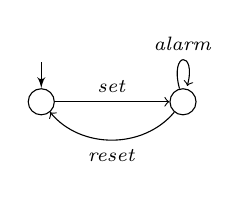
\begin{tikzpicture}[font=\sffamily\scriptsize]
        \node[vertex] (a) at (0, 0) {};
        \node[vertex] (b) at (1.8, 0) {};

        \draw[edge] (0, 0.5) to (a);
        \path[->] (a) edge  node[above] {$\mathit{set}$} (b);
        \path[->] (b) edge  [loop above] node {$\mathit{alarm}$} ();
        \path[->] (b) edge  [bend left=50] node[below] {$\mathit{reset}$} (a);
      \end{tikzpicture}
    \end{minipage}
    \begin{minipage}{.5\linewidth}
      \centering
      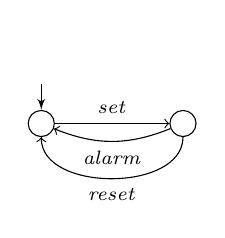
\begin{tikzpicture}[font=\sffamily\scriptsize]
        \node[vertex] (a) at (0, 0) {};
        \node[vertex] (b) at (1.8, 0) {};
        \node at (0, 1.1) {};

        \draw[edge] (0, 0.5) to (a);
        \path[->] (a) edge  node[above] {$\mathit{set}$} (b);
        \path[->] (b) edge  [bend left=22] node[below] {$\mathit{alarm}$} (a);
        \path[->] (b) edge  [bend left=90] node[below] {$\mathit{reset}$} (a);
      \end{tikzpicture}
    \end{minipage}
  \end{tabular} \\[12pt]

  In the two figures above you can see examples of two LTSs for alarm clocks. The first alarm clock on the left allows for repeated alarms which can be seen by the loop on top of the alarm state. With the second alarm clock it is only possible to signal the alarm once. \\
  Both LTSs are determistic since no state has more than one outgoing transition with the same label to a different state. However we can make the right LTS nondeterministic by drawing a loop on top of the alarm state as you can see in the figure below. \\

  \begin{center}
    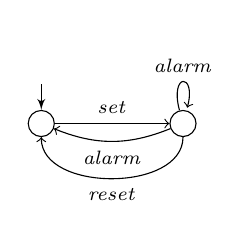
\begin{tikzpicture}[font=\sffamily\scriptsize]
      \node[vertex] (a) at (0, 0) {};
      \node[vertex] (b) at (1.8, 0) {};
      \node at (0, 1.1) {};

      \draw[edge] (0, 0.5) to (a);
      \path[->] (a) edge  node[above] {$\mathit{set}$} (b);
      \path[->] (b) edge  [bend left=22] node[below] {$\mathit{alarm}$} (a);
      \path[->] (b) edge  [loop above] node {$\mathit{alarm}$} ();
      \path[->] (b) edge  [bend left=90] node[below] {$\mathit{reset}$} (a);
    \end{tikzpicture}
  \end{center}

  \subsection{Bisimulation}
  Bisimulation is a binary relation between LTSs, where LTSs behave the same way in the sense
  that one LTS simulates the other and vice versa. Bisimulation is not the only form of equivalence. We can further differentiate between

  \begin{itemize}[noitemsep]
    \item Trace equivalence: \\
    Two LTSs are equivalent iff they can perform the same sequences of actions, starting from their initial states \\
    \item Strong bisimilarity: \\
    If one LTS can perform an action a then the other LTS must also be able to perform an action a in a way that the resulting states are again related. \\
  \end{itemize}

  Bisimilarity of two coffee machines: \\[18pt]
  \resizebox{\textwidth}{!}{
    \begin{tabular}{cc}
        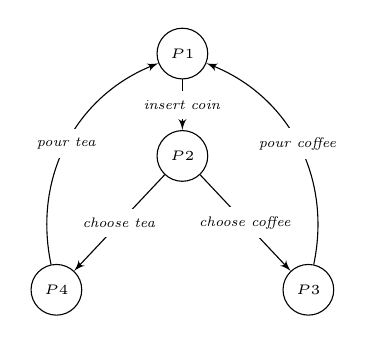
\begin{tikzpicture}[font=\sffamily\tiny]
          \node[vertex] (P1) at (1.6, 3) {$P1$};
          \node[vertex] (P2) at (1.6, 1.7) {$P2$};
          \node[vertex] (P3) at (3.2, 0) {$P3$};
          \node[vertex] (P4) at (0, 0) {$P4$};

          \path[edge] (P1) edge node[fill=white] {$\mathit{insert\ coin}$} (P2);
          \path[edge] (P2) edge node[fill=white] {$\mathit{choose\ coffee}$} (P3);
          \path[edge] (P2) edge node[fill=white] {$\mathit{choose\ tea}$} (P4);
          \path[edge] (P3) edge [bend right=40] node[fill=white] {$\mathit{pour\ coffee}$} (P1);
          \path[edge] (P4) edge [bend left=40] node[fill=white] {$\mathit{pour\ tea}$} (P1);
        \end{tikzpicture}
        &
        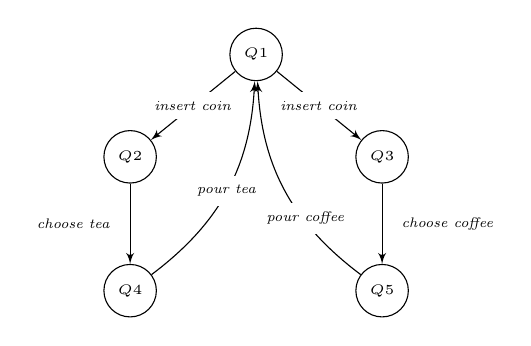
\begin{tikzpicture}[font=\sffamily\tiny]
          \node[vertex] (Q1) at (1.6, 3) {$Q1$};
          \node[vertex] (Q2) at (0, 1.7) {$Q2$};
          \node[vertex] (Q3) at (3.2, 1.7) {$Q3$};
          \node[vertex] (Q4) at (0, 0) {$Q4$};
          \node[vertex] (Q5) at (3.2, 0) {$Q5$};

          \path[edge] (Q1) edge node[fill=white] {$\mathit{insert\ coin}$} (Q2);
          \path[edge] (Q1) edge node[fill=white] {$\mathit{insert\ coin}$} (Q3);
          \path[edge] (Q2) edge node[label=left:$\mathit{choose\ tea}$] {} (Q4);
          \path[edge] (Q3) edge node[label=right:$\mathit{choose\ coffee}$] {} (Q5);
          \path[edge] (Q4) edge [bend right=25] node[fill=white] {$\mathit{pour\ tea}$} (Q1);
          \path[edge] (Q5) edge [bend left=25]  node[xshift=7.5pt, yshift=-10pt, fill=white] {$\mathit{pour\ coffee}$} (Q1);
        \end{tikzpicture}
    \end{tabular}
  } \\[8pt]

  The two coffee machines in the figures above are trace equivalent but not strongly bisimilar because the resulting states are not related. As an example we can check what happens after inserting a coin. With the first coffee machine we reach state $P2$ and with the second coffee machine we reach either $Q2$ or $Q3$ depending on the choice of beverage.\\
  So the process of inserting a coin and then either getting a coffee or a tea is the same but the path on how we get there is different.

  \section{µ-Calculus}
  As already mentioned before µ-Calculus is an integral part of $mcrl2$. µ-Calculus is an extension of propositional logic and therefore shares some similiarites. \\
  Furthermore it is used to describe and verify properties of LTSs.

  \subsection{Hennessy-Milner Logic}
  \begin{align*}
    \phi ::= \mathit{true}\ |\ \mathit{false}\ |\ \neg \phi\ |\ \phi \land \psi\ |\ \phi \lor \psi\ |\ \phi \to \psi\ |\ \langle a \rangle \phi \ |\ [a]\phi
  \end{align*}
  \begin{itemize}
    \item $\mathit{true}$ is true in each state of a process and $\mathit{false}$ is never true
    \item $\neg ,\ \land\ ,\ \lor$ and $\to$ as in propositional logic
    \item $\langle a \rangle \phi$ is valid whenever an $a-action$ can be performed such that $\phi$ is valid after this $a$ has been done
    \item $[a]\phi$ is valid when for every action $a$ that can be done, $\phi$ holds after doing that $a$
  \end{itemize}

  \subsection{Diamond and Box Modalities}

  Although $\langle a \rangle \phi$ - diamond modality and $[a]\phi$ - box modality look somewhat similar, yet they are very different. In order to show the difference between the two modalities we have four simple LTSs where we take look wheter the box modality or the diamond modality of $a$.

  \resizebox{\textwidth}{!}{
    \newcommand{\valid}{{\color{green} valid}}
    \newcommand{\invalid}{{\color{red} invalid}}
    \renewcommand{\arraystretch}{2}
    \begin{tabular}{l c c c c}
      &

      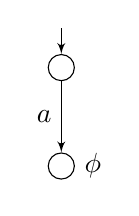
\begin{tikzpicture}
        \node[vertex] (a) at (0, 1.25) {};
        \node[vertex] [label=right:{$\phi$}] (b) at (0, 0) {};

        \draw[edge] (0, 1.75) to (a);
        \draw[edge] (a) to node [left] {$a$} (b);
      \end{tikzpicture}

      &

      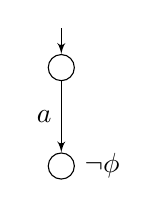
\begin{tikzpicture}
        \node[vertex] (a) at (0, 1.25) {};
        \node[vertex] [label=right:{$\neg\phi$}] (b) at (0, 0) {};

        \draw[edge] (0, 1.75) to (a);
        \draw[edge] (a) to node [left] {$a$} (b);
      \end{tikzpicture}

      &

      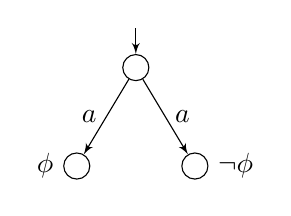
\begin{tikzpicture}
        \node[vertex] (a) at (0.75, 1.25) {};
        \node[vertex] [label=left:{$\phi$}] (b) at (0, 0) {};
        \node[vertex] [label=right:{$\neg\phi$}] (c) at (1.5, 0) {};

        \draw[edge] (.75, 1.75) to (a);
        \draw[edge] (a) to node [left] {$a$} (b);
        \draw[edge] (a) to node [right] {$a$} (c);
      \end{tikzpicture}

      &

      \begin{tikzpicture}
        \node[vertex] (a) at (0, 1.25) {};
        \node at (0, -0.175) {};

        \draw[edge] (0, 1.75) to (a);
      \end{tikzpicture}

      \\

      $\langle{}a\rangle{}\phi$ & \valid & \invalid & \valid & \invalid \\

      $[a]\phi$                 & \valid & \invalid & \invalid &  \valid \\
    \end{tabular}
  }\\[6pt]

  In the first LTS a $a$ action is possible to a state where $\phi$ holds and therefore both $\langle{}a\rangle{}\phi$ and $[a]\phi$ are possible. \\
  In the second LTS there is no $a$ action to a state where $\phi$ holds and for that reason both $\langle{}a\rangle{}\phi$ and $[a]\phi$ are not possible. \\
  In the third LTS there is no $a$ action to a state where $\phi$ holds and an $a$ action to a state where $\phi$ does not holds and therefore $\langle{}a\rangle{}\phi$ is valid since there is at least one $a$ action that leads to a valid $\phi$ and $[a]\phi$ is not valid because not every $a$ action results in a valid $[a]\phi$. \\
  In the fourth LTS there is no $a$ action at all and therefore $\langle{}a\rangle{}\phi$ is not valid because, because there needs to be an $a$ action that can be performed and $[a]\phi$ is valid, since there is no action that can be done. \\
\end{document}
